\section{Coleta de dados e simulação do ambiente musical \textit{online}}

Para realizar os experimentos, procuramos simular, de forma simples, um ambiente colaborativo musical \textit{online} \textit{peer-to-peer}, do ponto de vista do músico local. Nosso conjunto de dados, dessa forma, contém pares de arquivos de música com as seguintes regras:

\begin{enumerate}
    \item Ambos reproduzem a mesma sequência de uma música, porém, em performances diferentes;
    \item Ambos consistem de apenas um instrumento;
    \item Ambos consistem do mesmo instrumento.
\end{enumerate}

A regra 1 visa simular a transmissão de dados - é importante que os arquivos reproduzam a mesma sessão da música, porém, de formas diferentes, como um ser humano faria. A regra 2, apesar de não obrigatória em transmissões em casos reais, simplifica o processamento e previsão dos áudios; além disso, não é esperado que vários músicos compartilhem do mesmo canal de transmissão. Por último, a regra 3 complementa a as duas regras anteriores, garantindo a mesma sequência de áudio performada de diferentes maneiras pelo mesmo instrumento.

Para cada par, podemos nomear o primeiro arquivo $A$ e o segundo $B$, onde $A$ é classificado como o conjunto de treinamento o $B$ o conjunto de teste. Dessa forma, conseguimos simular um ambiente onde um dos músicos possui o conjunto $A$ treinado em sua máquina e está recebendo o conjunto $B$ do músico remoto.

Para coletar arquivos com esses requisitos, a seguinte abordagem foi realizada, ilustrada na \figref{fig:data_gathering}: (1) buscou-se músicas onde a mesma sequência de acordes e notas era reproduzida em diferentes sessões (por exemplo, uma introdução que serve de motivo para a música); (2) depois, isolou-se apenas um instrumento; (3) identificou-se as sessões repetidas e; (4) separou-se as sessões isoladamente e criou-se os dois arquivos, um para treinamento e outro para simulação do áudio remoto.

\begin{figure}[htbp]
\centering
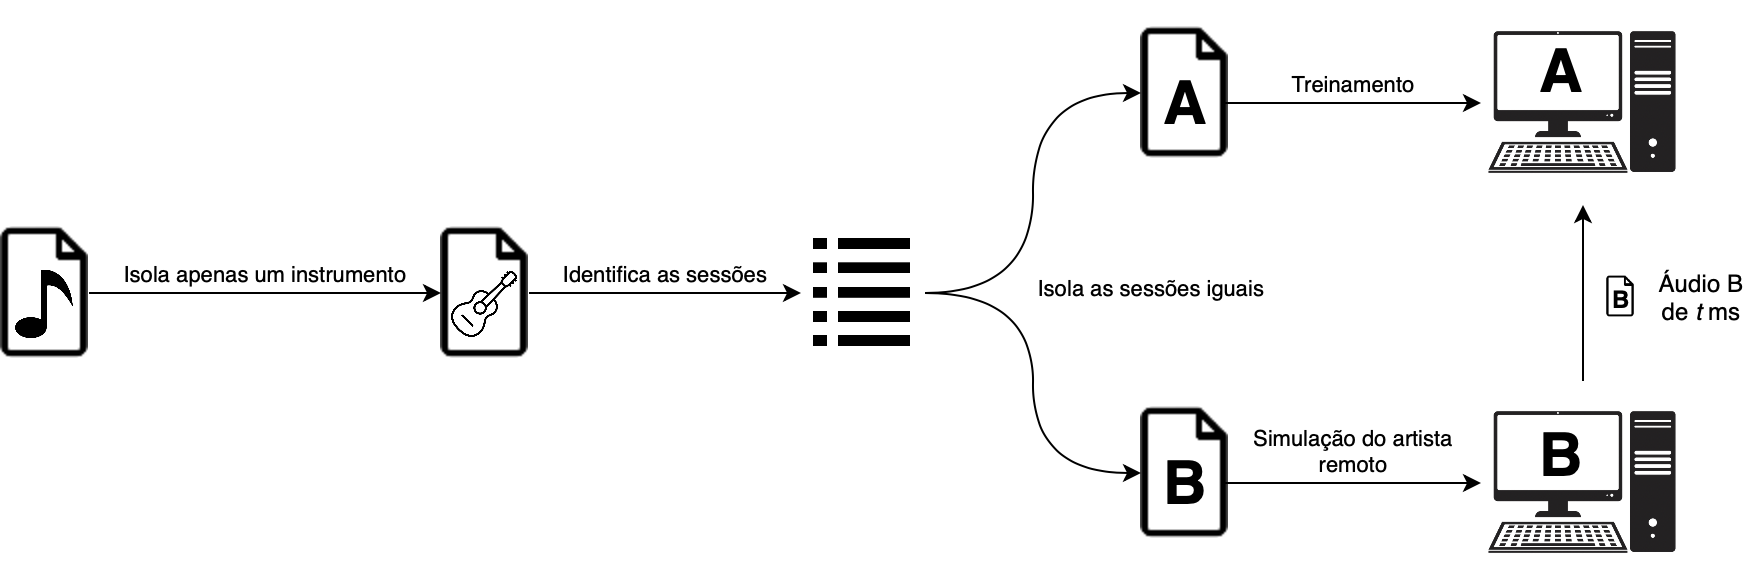
\includegraphics[width=1\textwidth]{images/data-gathering.png}
\caption{Processo de coleta de dados e simulação de um ambiente musical colaborativo \textit{peer-to-peer}.}
\label{fig:data_gathering}
\end{figure}

Essa metodologia de separação de arquivos implica em dizer que a adaptação proposta não pode utilizar nenhum dado futuro do arquivo $B$, pois, no ambiente real, essa informação também não estaria presente. O arquivo $A$, por sua vez, pode ser analisado integralmente. Inclusive, tal análise pode ser realizada em momento anterior às previsões, já que o único tempo relevante a ser metrificado é o que foi levado para gerá-las. Em um ambiente real, o treinamento pode ser realizado antes que os músicos toquem juntos.

As músicas utilizadas nos experimentos foram \textit{Hotel California} (\textit{Eagles}, 1976) - tendo a trilha do violão acústico isolada - e \textit{Message In A Bottle} (\textit{The Police}, 1979) - onde a trilha da guitarra elétrica de base foi isolada.
